\homework{5}{Thu 15 Sep 2022 21:33}{Week 5 due Sep 27}

\begin{enumerate}
	\item 
		p. 130: 3 Find a solution to the boundary value problem depicted in Fig. $3.13$ and evaluate it at $(1,1)$.
\begin{figure}[H]
	\centering
	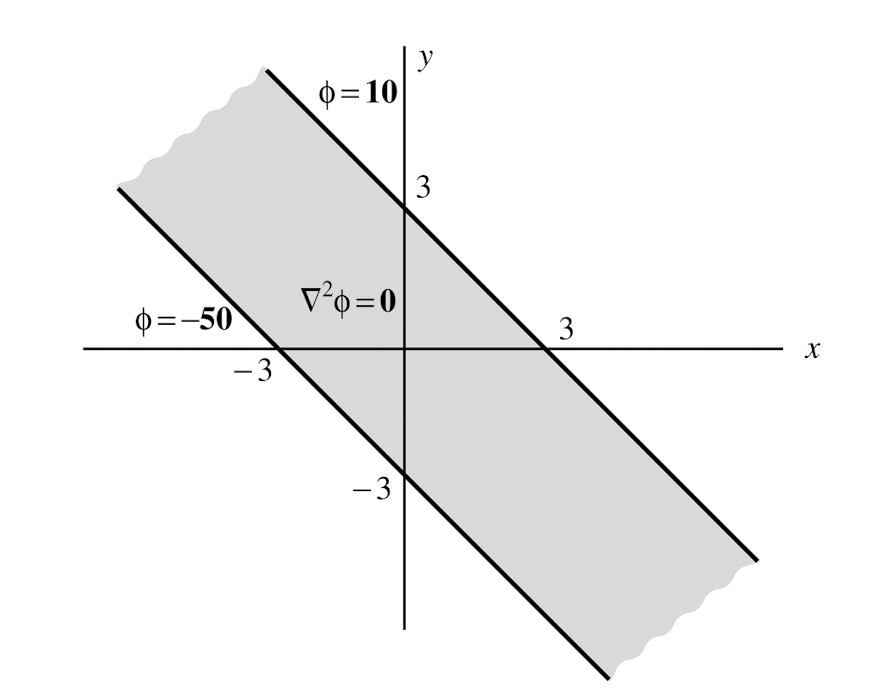
\includegraphics[width=0.8\textwidth]{figures/ex3.4p3.png}
	\caption{problem 3}
\end{figure}
\begin{proof}[Solution]
Denote the region as $\mathcal{D}$. The boundary $\partial \mathcal{D} = A \cup B$ where
\begin{align*}
	A &= \{t-it-3i: t \in \mathbb{R}\}  \\
	B &= \{t-it+3i: t \in \mathbb{R}\} 
.\end{align*}
We define the mapping 
\begin{align*}
	f: \mathcal{D} &\longrightarrow \mathcal{D}_0 \\
	z &\longmapsto f(z) = a z + b
\end{align*}
where 
\begin{align*}
	\operatorname{Im} f(A) &= 0 \\
	\operatorname{Im} f(B) &= 1
.\end{align*}

There exists a solution
\begin{align*}
	a &=  \frac{1}{6}(1+i)\\
	b &= \frac{1}{2}i
.\end{align*}

Now $f$ maps $\mathcal{D}$ to the simpler region \[ 
	\mathcal{D}_0 = \{z:0< \operatorname{Im} z <1\} 
.\] 
Also, $f$ maps $\partial \mathcal{D}$ to $\partial \mathcal{D}_0$. It maps $A$ to $A_0$,  the real axis, and  $B$ to $B_0$, the line $Im z = 1$.

Now we solve the simpler boundary problem:

We have  $\varphi = -50$ on $A_0$ and $\varphi = 10$ on $B_0$. It is assumed that $\nabla^2 \varphi = 0$. Parameterize $\varphi$ by \[
	\varphi(x + i y) = b y + c
.\] 
Now plug in boundary conditions:
\[
	\begin{cases}
		b(0) + c =  -50\\
		b(1) + c = 10
	\end{cases}
\]
Hence \[
	\begin{cases}
		b = 60\\
		c = -50
	\end{cases}
.\] 

To get the solution to original boundary problem, note 
\begin{align*}
	\Phi(z) &= \varphi \circ f (z)\\
	&= \varphi(\frac{1}{6}(1+i)z + \frac{1}{2}i) \\
	&= 60 \operatorname{Im} \left(\frac{1}{6}(1+i)z + \frac{1}{2}i\right) - 50
.\end{align*}
Evaluate at  $z = 1 + i$ :
\begin{align*}
	\Phi(1+i) &=  60 \operatorname{Im} \left(\frac{1}{6}(1+i)z + \frac{1}{2}i\right) - 50\\
	&=  60 \operatorname{Im} \left(\frac{1}{6}(1+i)(1+i) + \frac{1}{2}i\right) - 50\\
	&=  60 \operatorname{Im} \left(\frac{1}{6}(2i) + \frac{1}{2}i\right) - 50\\
	&=  60 \operatorname{Im} \left(\frac{5}{6}i\right) - 50\\
	&= 0
.\end{align*}
\end{proof}
\newpage
\item 4 Solve the boundary problem.
\begin{figure}[H]
	\centering
	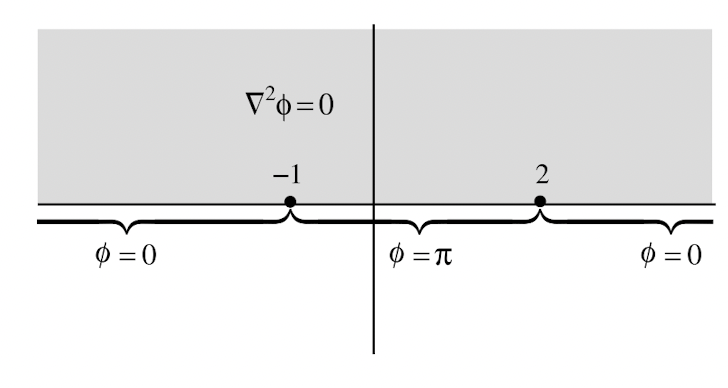
\includegraphics[width=0.8\textwidth]{figures/ex3.4p4.png}
	\caption{problem 4}
\end{figure}
\begin{proof}[Solution]
	The solution is of the form \[
		\Phi(z) = p\operatorname{Arg} (z-2) + q \operatorname{Arg} (z+1)
	.\] 
	Where \[
		p = 1, q = -1
	.\] 
	Evaluate at $(2,3)$ :
	\begin{align*}
		\Phi(2+3i) &= \operatorname{Arg} (2+3i-2) - \operatorname{Arg} (2+3 i + 1) \\
		&= \operatorname{Arg} (3i) - \operatorname{Arg} (3+3 i) \\
		&= \frac{\pi}{2} - \frac{\pi}{4} \\
		&= \frac{\pi}{4}
	.\end{align*} 
\end{proof}

\item p. 136: 1(abd),

\item 15(a);
\item p. 160: 3,
\item 8;
\item p. 170: 3(ab),
\item 8,
\item 13,
\item p. 178: 1(a-e),
\item 4.

\end{enumerate}
